\documentclass[aspectratio=169]{beamer}
\usepackage[T1]{fontenc}
\usepackage{lmodern}
\usepackage{booktabs}
\usepackage{array}
\usepackage{tikz}
\usetikzlibrary{positioning, arrows.meta, shapes.geometric, fit, calc}
\usetheme{metropolis}
\usefonttheme{professionalfonts}
\setbeamertemplate{footline}[frame number]
\setbeamerfont{frametitle}{size=\large}
\setbeamertemplate{navigation symbols}{}

\title{ARC-AGI-3 Symbolica Research}
\subtitle{Runtime flow and current failure mode on \texttt{ls20}}
\author{ARC-AGI-3 Symbolica Research}
\date{}

\definecolor{BlueA}{HTML}{1F4E79}
\definecolor{BlueB}{HTML}{DCEAF7}
\definecolor{GreenA}{HTML}{2D7D46}
\definecolor{GreenB}{HTML}{E3F3E7}
\definecolor{OrangeA}{HTML}{B56A1E}
\definecolor{OrangeB}{HTML}{F7E9D6}
\definecolor{RedA}{HTML}{A33636}
\definecolor{RedB}{HTML}{F7DEDE}
\definecolor{GrayA}{HTML}{5F6368}
\definecolor{GrayB}{HTML}{EEF1F4}

\tikzset{
  box/.style={draw, rounded corners=2pt, align=center, font=\scriptsize, minimum height=0.95cm, inner sep=4pt},
  soft/.style={fill=GrayB, draw=black!35},
  wm/.style={fill=BlueB, draw=BlueA},
  dc/.style={fill=GreenB, draw=GreenA},
  rt/.style={fill=OrangeB, draw=OrangeA},
  bad/.style={fill=RedB, draw=RedA},
  arr/.style={-{Latex[length=1.7mm]}, thick},
  note/.style={draw, rounded corners=2pt, fill=white, align=left, font=\scriptsize, inner sep=4pt}
}

\begin{document}

\begin{frame}[plain]
  \titlepage
\end{frame}

\begin{frame}{Why this framework was added}
\centering
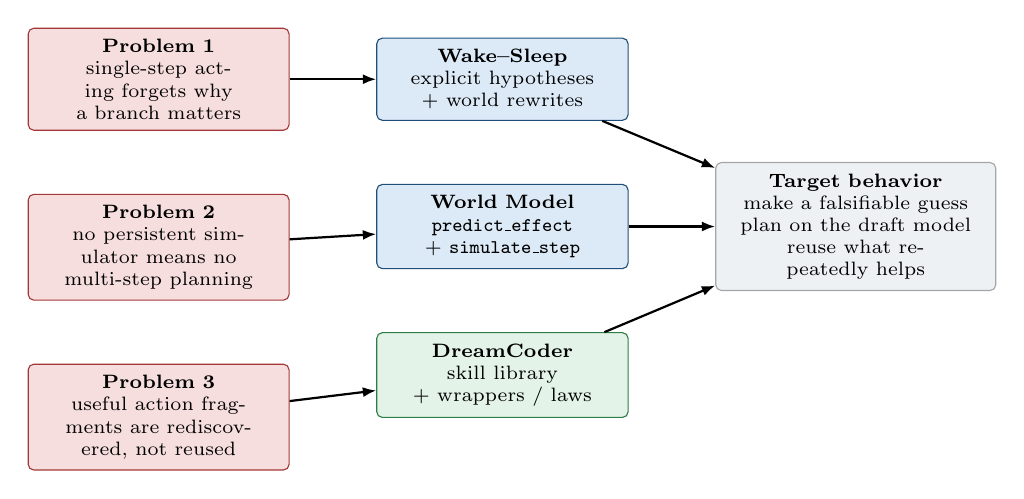
\begin{tikzpicture}[node distance=0.8cm and 0.8cm]
  \node[box,bad,text width=0.25\textwidth] (p1) {\textbf{Problem 1}\\single-step acting forgets why a branch matters};
  \node[box,bad,below=of p1,text width=0.25\textwidth] (p2) {\textbf{Problem 2}\\no persistent simulator means no multi-step planning};
  \node[box,bad,below=of p2,text width=0.25\textwidth] (p3) {\textbf{Problem 3}\\useful action fragments are rediscovered, not reused};

  \node[box,wm,right=1.1cm of p1,text width=0.24\textwidth] (m1) {\textbf{Wake--Sleep}\\explicit hypotheses\\+ world rewrites};
  \node[box,wm,below=of m1,text width=0.24\textwidth] (m2) {\textbf{World Model}\\\texttt{predict\_effect}\\+ \texttt{simulate\_step}};
  \node[box,dc,below=of m2,text width=0.24\textwidth] (m3) {\textbf{DreamCoder}\\skill library\\+ wrappers / laws};

  \node[box,soft,right=1.1cm of m2,text width=0.27\textwidth] (goal) {\textbf{Target behavior}\\make a falsifiable guess\\plan on the draft model\\reuse what repeatedly helps};

  \draw[arr] (p1) -- (m1);
  \draw[arr] (p2) -- (m2);
  \draw[arr] (p3) -- (m3);
  \draw[arr] (m1) -- (goal);
  \draw[arr] (m2) -- (goal);
  \draw[arr] (m3) -- (goal);
\end{tikzpicture}
\end{frame}

\begin{frame}{Runtime map in code}
\centering
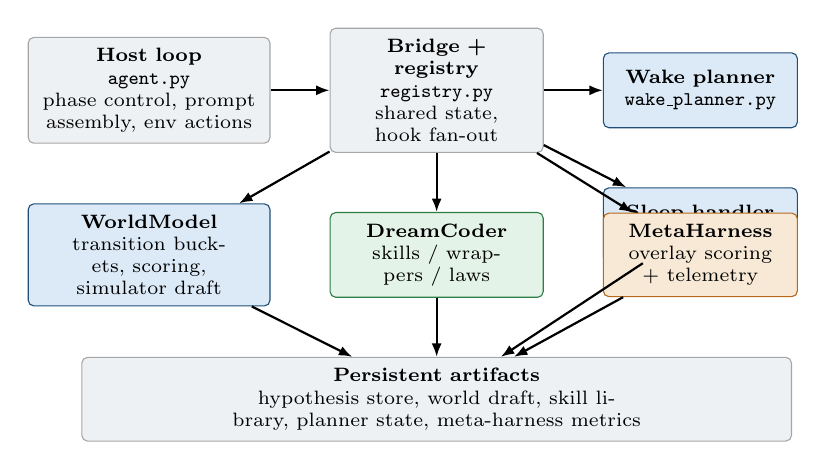
\begin{tikzpicture}[node distance=0.75cm and 0.75cm]
  \node[box,soft,text width=0.23\textwidth] (agent) {\textbf{Host loop}\\\texttt{agent.py}\\phase control, prompt assembly, env actions};
  \node[box,soft,right=of agent,text width=0.2\textwidth] (registry) {\textbf{Bridge + registry}\\\texttt{registry.py}\\shared state, hook fan-out};
  \node[box,wm,right=of registry,text width=0.18\textwidth] (wake) {\textbf{Wake planner}\\\texttt{wake\_planner.py}};
  \node[box,wm,below=of wake,text width=0.18\textwidth] (sleep) {\textbf{Sleep handler}\\\texttt{sleep\_handler.py}};
  \node[box,dc,below=of registry,text width=0.2\textwidth] (dcmod) {\textbf{DreamCoder}\\skills / wrappers / laws};
  \node[box,wm,left=of dcmod,text width=0.23\textwidth] (wmmod) {\textbf{WorldModel}\\transition buckets, scoring, simulator draft};
  \node[box,rt,right=of dcmod,text width=0.18\textwidth] (meta) {\textbf{MetaHarness}\\overlay scoring + telemetry};
  \node[box,soft,below=of dcmod,text width=0.72\textwidth] (persist) {\textbf{Persistent artifacts}\\hypothesis store, world draft, skill library, planner state, meta-harness metrics};

  \draw[arr] (agent) -- (registry);
  \draw[arr] (registry) -- (wake);
  \draw[arr] (registry) -- (sleep);
  \draw[arr] (registry) -- (wmmod);
  \draw[arr] (registry) -- (dcmod);
  \draw[arr] (registry) -- (meta);
  \draw[arr] (wmmod) -- (persist);
  \draw[arr] (dcmod) -- (persist);
  \draw[arr] (meta) -- (persist);
  \draw[arr] (sleep) -- (persist);
\end{tikzpicture}
\end{frame}

\begin{frame}{One online cycle}
\centering
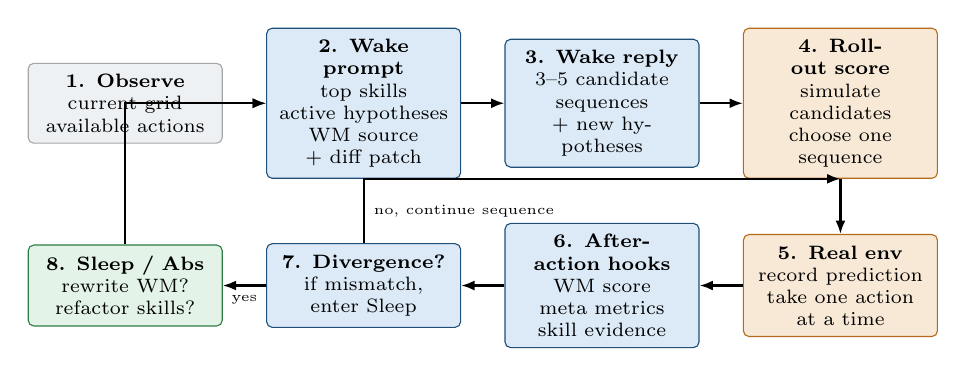
\begin{tikzpicture}[node distance=0.7cm and 0.55cm]
  \node[box,soft,text width=0.18\textwidth] (s1) {\textbf{1. Observe}\\current grid\\available actions};
  \node[box,wm,right=of s1,text width=0.18\textwidth] (s2) {\textbf{2. Wake prompt}\\top skills\\active hypotheses\\WM source + diff patch};
  \node[box,wm,right=of s2,text width=0.18\textwidth] (s3) {\textbf{3. Wake reply}\\3--5 candidate sequences\\+ new hypotheses};
  \node[box,rt,right=of s3,text width=0.18\textwidth] (s4) {\textbf{4. Rollout score}\\simulate candidates\\choose one sequence};

  \node[box,rt,below=of s4,text width=0.18\textwidth] (s5) {\textbf{5. Real env}\\record prediction\\take one action at a time};
  \node[box,wm,left=of s5,text width=0.18\textwidth] (s6) {\textbf{6. After-action hooks}\\WM score\\meta metrics\\skill evidence};
  \node[box,wm,left=of s6,text width=0.18\textwidth] (s7) {\textbf{7. Divergence?}\\if mismatch, enter Sleep};
  \node[box,dc,left=of s7,text width=0.18\textwidth] (s8) {\textbf{8. Sleep / Abs}\\rewrite WM?\\refactor skills?};

  \draw[arr] (s1) -- (s2);
  \draw[arr] (s2) -- (s3);
  \draw[arr] (s3) -- (s4);
  \draw[arr] (s4) -- (s5);
  \draw[arr] (s5) -- (s6);
  \draw[arr] (s6) -- (s7);
  \draw[arr] (s7) -- node[below,font=\tiny]{yes} (s8);
  \draw[arr] (s8) |- (s2);
  \draw[arr] (s7.north) |- node[pos=0.25,right,font=\tiny]{no, continue sequence} (s4.south);
\end{tikzpicture}

\vspace{0.35em}
\small
This is the active path in \texttt{ArcgenticaResearch}: online control is Wake $\rightarrow$ real env $\rightarrow$ Sleep, not pure MCTS.
\end{frame}

\begin{frame}{What enters one Wake call}
\small
\begin{columns}[T,totalwidth=\textwidth]
\begin{column}{0.5\textwidth}
\begin{block}{Input blocks from code}
\begin{itemize}
\item current grid snapshot
\item available action names
\item top-3 retrieved skills
\item active hypotheses from the frontier
\item world-model source summary
\item last divergence summary
\item movement summary + changed cells
\item initial-frame summary + amplified diff patch
\end{itemize}
\end{block}
\end{column}
\begin{column}{0.5\textwidth}
\begin{block}{Expected Wake output}
\begin{itemize}
\item candidate sequences
\item rationale
\item referenced skills
\item 0--3 new falsifiable hypotheses
\end{itemize}
\end{block}
\vspace{0.4em}
\begin{block}{Why this matters}
The prompt is no longer ``what action next?''\\
It is ``what sequence and what hypothesis should the runtime test next?''
\end{block}
\end{column}
\end{columns}
\end{frame}

\begin{frame}{What happens after one real action}
\centering
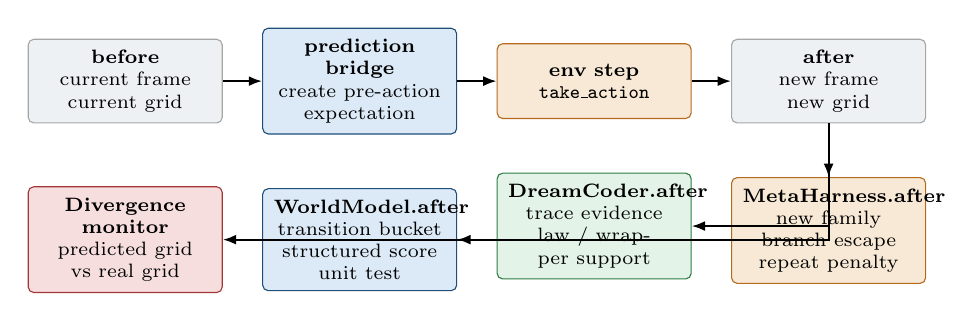
\begin{tikzpicture}[node distance=0.68cm and 0.5cm]
  \node[box,soft,text width=0.18\textwidth] (a1) {\textbf{before}\\current frame\\current grid};
  \node[box,wm,right=of a1,text width=0.18\textwidth] (a2) {\textbf{prediction bridge}\\create pre-action expectation};
  \node[box,rt,right=of a2,text width=0.18\textwidth] (a3) {\textbf{env step}\\\texttt{take\_action}};
  \node[box,soft,right=of a3,text width=0.18\textwidth] (a4) {\textbf{after}\\new frame\\new grid};

  \node[box,wm,below=of a2,text width=0.18\textwidth] (a5) {\textbf{WorldModel.after}\\transition bucket\\structured score\\unit test};
  \node[box,dc,below=of a3,text width=0.18\textwidth] (a6) {\textbf{DreamCoder.after}\\trace evidence\\law / wrapper support};
  \node[box,rt,below=of a4,text width=0.18\textwidth] (a7) {\textbf{MetaHarness.after}\\new family\\branch escape\\repeat penalty};
  \node[box,bad,left=of a5,text width=0.18\textwidth] (a8) {\textbf{Divergence monitor}\\predicted grid vs real grid};

  \draw[arr] (a1) -- (a2);
  \draw[arr] (a2) -- (a3);
  \draw[arr] (a3) -- (a4);
  \draw[arr] (a4) |- (a5);
  \draw[arr] (a4) -- (a7);
  \draw[arr] (a4) |- (a6);
  \draw[arr] (a4) |- (a8);
\end{tikzpicture}

\vspace{0.35em}
\small
The key fix in recent code was to restore this prediction bridge on the Rev M path so WorldModel can score expected vs actual transitions.
\end{frame}

\begin{frame}{Online action selection vs optional MCTS}
\small
\begin{columns}[T,totalwidth=\textwidth]
\begin{column}{0.49\textwidth}
\begin{block}{Actual online path now}
\begin{itemize}
\item Wake LLM sees grid, hypotheses, skills, diff patch
\item it proposes 3--5 action sequences
\item runtime scores those sequences on the current world draft
\item chosen sequence is executed in the real environment
\end{itemize}
\end{block}
\begin{block}{Meaning}
The online agent is already much closer to\\
\textbf{``LLM writes the test sequence''}\\
than to classical tree search.
\end{block}
\end{column}
\begin{column}{0.49\textwidth}
\begin{block}{Optional MCTS side path}
\begin{itemize}
\item lives in \texttt{planner.py}
\item opens only when WM gate says the draft is good enough
\item still uses UCB1 selection on the search tree
\item may commit top paths into DreamCoder as skills
\end{itemize}
\end{block}
\begin{block}{Meaning}
UCB is still present, but it is \textbf{not} the main online control path.
\end{block}
\end{column}
\end{columns}
\end{frame}

\begin{frame}{Module inputs and outputs}
\centering
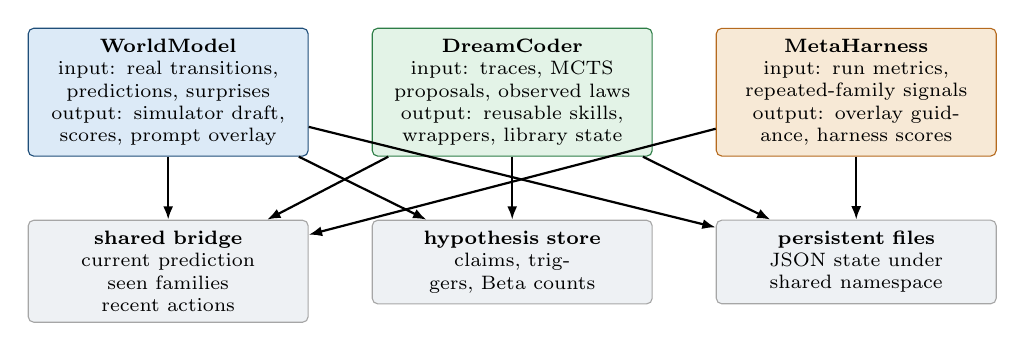
\begin{tikzpicture}[node distance=0.8cm and 0.8cm]
  \node[box,wm,text width=0.27\textwidth] (wm) {\textbf{WorldModel}\\input: real transitions, predictions, surprises\\output: simulator draft, scores, prompt overlay};
  \node[box,dc,right=of wm,text width=0.27\textwidth] (dc) {\textbf{DreamCoder}\\input: traces, MCTS proposals, observed laws\\output: reusable skills, wrappers, library state};
  \node[box,rt,right=of dc,text width=0.27\textwidth] (mh) {\textbf{MetaHarness}\\input: run metrics, repeated-family signals\\output: overlay guidance, harness scores};

  \node[box,soft,below=of wm,text width=0.27\textwidth] (h1) {\textbf{shared bridge}\\current prediction\\seen families\\recent actions};
  \node[box,soft,below=of dc,text width=0.27\textwidth] (h2) {\textbf{hypothesis store}\\claims, triggers, Beta counts};
  \node[box,soft,below=of mh,text width=0.27\textwidth] (h3) {\textbf{persistent files}\\JSON state under shared namespace};

  \draw[arr] (wm) -- (h1);
  \draw[arr] (dc) -- (h1);
  \draw[arr] (mh) -- (h1);
  \draw[arr] (wm) -- (h2);
  \draw[arr] (dc) -- (h2);
  \draw[arr] (wm) -- (h3);
  \draw[arr] (dc) -- (h3);
\draw[arr] (mh) -- (h3);
\end{tikzpicture}
\end{frame}

\begin{frame}{Real hypothesis examples from the store}
\scriptsize
\begin{columns}[T,totalwidth=\textwidth]
\begin{column}{0.5\textwidth}
\begin{block}{Example A: generic seed goal}
\textbf{Claim}\\
\texttt{[L0] A sequence of available actions reaches WIN.}

\vspace{0.25em}
\textbf{Status}\\
active, \texttt{is\_goal=True}, support 0 / falsify 7

\vspace{0.25em}
\textbf{Why it is weak}\\
It states the existence of a solve path, but says nothing about the actual mechanic.
\end{block}
\end{column}
\begin{column}{0.5\textwidth}
\begin{block}{Example B: currently common mechanic hypothesis}
\textbf{Claim}\\
\texttt{ACTION4 typically causes a large grid change.}

\vspace{0.25em}
\textbf{Trigger}\\
\texttt{after ACTION4}

\vspace{0.25em}
\textbf{Meaning}\\
This is measurable and often confirmed, but it explains redraw magnitude, not goal progress.
\end{block}
\end{column}
\end{columns}

\vspace{0.35em}
\begin{block}{Short check-code example}
\texttt{if action != 'ACTION4': result = None}\\
\texttt{else: compare before/after summaries and treat large remap as support}
\end{block}
\end{frame}

\begin{frame}[fragile]{Real world-model code example}
\scriptsize
\begin{block}{Persisted \texttt{predict\_effect(action, observation)} draft}
\begin{verbatim}
def predict_effect(action, observation):
    sig = observation.get('signature', '')
    if sig == 'd2072020114e7cd91549' and action in ('ACTION2','ACTION4'):
        return {
            'expect_change': True,
            'expected_diff_band': 'large',
            'expected_next_grid': new_grid,
            'latent_state_prediction': {...},
            'goal_progress_prediction': {'progress_delta': 0.0}
        }
\end{verbatim}
\end{block}

\begin{block}{What this tells us}
The draft is executable code and already emits latent / goal fields, but the logic is still mostly empirical replay of observed deltas, not a compact mechanic simulator.
\end{block}
\end{frame}

\begin{frame}{What changed from the naive world model}
\small
\centering
\begin{tabular}{p{0.29\textwidth} p{0.29\textwidth} p{0.29\textwidth}}
\toprule
\textbf{Before} & \textbf{Now} & \textbf{Meaning} \\
\midrule
one-step diff note & executable \texttt{predict\_effect} draft & planning can call the simulator \\
free-form notes & explicit hypotheses + strict checks & failure becomes local and patchable \\
action retry loops & Wake sequence + Sleep rewrite + abstraction & search has memory across turns \\
\bottomrule
\end{tabular}
\end{frame}

\begin{frame}{Plan lens: intent, hypothesis, verification}
\scriptsize
\centering
\begin{tabular}{p{0.23\textwidth} p{0.34\textwidth} p{0.34\textwidth}}
\toprule
\textbf{Intent} & \textbf{Hypothesis} & \textbf{Verification} \\
\midrule
Wake should test mechanics & richer input yields better sequences + falsifiable hypotheses & candidate count, accepted hypotheses, startup stability \\
World model should learn mechanics & prediction bridge + Sleep rewrite activate empirical scoring & structured prediction count, scored matches, world update \\
Planner should matter only after WM quality rises & optional MCTS stays gated until the draft is useful & gate reason, planner state, MCTS vs BFS advantage \\
Skill library should store reusable control & DreamCoder promotes wrappers / controllers, not raw fragments & skill mix: wrappers, laws, executable leaves \\
\bottomrule
\end{tabular}
\end{frame}

\begin{frame}{Recent bounded results mapped to the plan}
\small
\begin{columns}[T,totalwidth=\textwidth]
\begin{column}{0.48\textwidth}
\begin{block}{What the recent runs did prove}
\begin{itemize}
\item Wake startup is stable again
\item rate limiting is not the current blocker
\item goal/state hypotheses survive early turns more often
\item helper / whitelist mismatches were reduced
\end{itemize}
\end{block}
\end{column}
\begin{column}{0.48\textwidth}
\begin{block}{What the recent runs did \emph{not} prove}
\begin{itemize}
\item no level-up yet on \texttt{ls20}
\item no stable world-model rewrite handoff
\item no reliable structured-prediction scoring loop yet
\item MCTS is still mostly irrelevant online because the gate stays cold
\end{itemize}
\end{block}
\end{column}
\end{columns}

\vspace{0.4em}
\begin{block}{Direct readout from reports}
\begin{itemize}
\item \texttt{state\_goal} runs: \texttt{startup\_stalled=false}, \texttt{rate\_limited=false}
\item \texttt{worldscore\_20260420a}: \texttt{startup\_stalled=true}
\end{itemize}
\end{block}
\end{frame}

\begin{frame}{Why \texttt{ls20} still stalls}
\centering
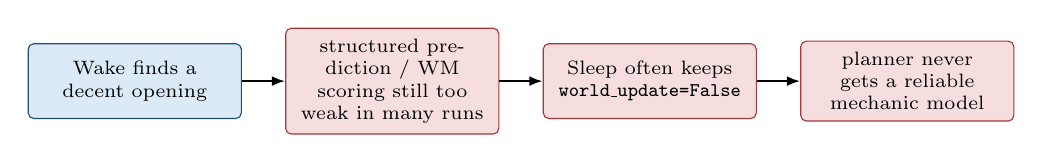
\begin{tikzpicture}[node distance=0.72cm and 0.55cm]
  \node[box,wm,text width=0.2\textwidth] (b1) {Wake finds a decent opening};
  \node[box,bad,right=of b1,text width=0.2\textwidth] (b2) {structured prediction / WM scoring still too weak in many runs};
  \node[box,bad,right=of b2,text width=0.2\textwidth] (b3) {Sleep often keeps\\\texttt{world\_update=False}};
  \node[box,bad,right=of b3,text width=0.2\textwidth] (b4) {planner never gets a reliable mechanic model};
  \draw[arr] (b1) -- (b2);
  \draw[arr] (b2) -- (b3);
  \draw[arr] (b3) -- (b4);
\end{tikzpicture}

\vspace{0.45em}
\small
So the runtime is better instrumented than before, but still fails at the exact handoff that should turn a good opening into a useful simulator rewrite.
\end{frame}

\begin{frame}{Next repair loop}
\small
\begin{columns}[T,totalwidth=\textwidth]
\begin{column}{0.33\textwidth}
\begin{block}{Intent}
Make the online loop produce a scored world-model correction, not just better telemetry.
\end{block}
\end{column}
\begin{column}{0.33\textwidth}
\begin{block}{Hypothesis}
If Rev M records structured predictions on the live action path, Sleep will finally receive evidence strong enough to rewrite the simulator draft.
\end{block}
\end{column}
\begin{column}{0.33\textwidth}
\begin{block}{Verification}
\begin{itemize}
\item \texttt{startup\_stalled = false}
\item structured prediction count moves above zero
\item empirical match/mismatch counts move
\item \texttt{world\_update = true} appears at least once
\end{itemize}
\end{block}
\end{column}
\end{columns}
\end{frame}

\end{document}
